\documentclass[12pt]{exam}
%-PACKAGES et MACROS nécessaires------------------------------------
\usepackage{enumitem}
\usepackage{dashrule}
\usepackage{tkz-euclide}
\def\doted#1{\hdashrule{#1}{.5pt}{2pt}}
\def\dotedline{\par\vspace{10pt}\hdashrule{\linewidth}{.5pt}{2pt}}
%-------------------------------------------------------------------

\begin{document}
    \begin{questions}
    \question
	\begin{parts}
		\part Soient%
			\par$\bullet$\quad ABC tel que AB = 5 cm, BC = 6 cm et AC = 8,5 cm~;
			\par$\bullet$\quad DEF tel que DE = 3 cm, EF = 7 cm et FD = 3,5 cm.
		\begin{subparts}
            \subpart Bnjour
			% \subpart Parmi ces deux triangles, un seul est constructible. Lequel ? Justifier la réponse.
			% \dotedline\dotedline\dotedline\dotedline\dotedline
			% \subpart Construire ce triangle (la précision du tracé est prise en compte dans la notation).
			% \vskip100pt
		\end{subparts}
		\part Voici deux autres triangles tracés à main levée. Lequel est constructible ? Justifier la réponse.
	\end{parts}
    \question
    \begin{parts}
        \part Calculer en détaillant les étapes.\par\medskip
        ${\rm A}=6+4\times25-5$\vskip100pt
        ${\rm B}=12\div4\times3$\vskip100pt
        ${\rm C}=6\times(13-(5-2))$\vskip100pt
        ${\rm D}=((8-2)\times8)\div4+8$\vskip100pt
    \end{parts}
    \question
    
    \question
    Préciser dans chaque cas ci dessous, si les droites (d$_1$) et (d$_2$) sont parallèles. Justifier la réponse.\par\noindent
    \hbox{\hbox to.5\linewidth{a)%
    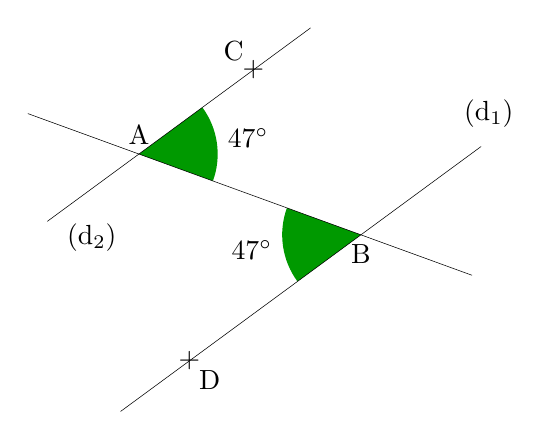
\begin{tikzpicture}[rotate=-20,baseline=(C.base)]
        \coordinate[label=above:A](A)at(0,0);
        \coordinate[label=below:B](B)at(3,0);
        \coordinate[label=above left:C](C)at(1,1.5);
        \coordinate[label=below right:D](D)at(1.5,-2.25);
        \draw node at(C){+};
        \draw node at(D){+};
        \tkzFillAngle[fill=green!60!black](B,A,C)
        \tkzLabelAngle[pos=1.4](B,A,C){$47^\circ$}
        \tkzFillAngle[fill=green!60!black](A,B,D)
        \tkzLabelAngle[pos=1.4](A,B,D){$47^\circ$}
        \tkzDrawLine[add=0.8 and 0.5](A,C)
        \tkzDrawLine[add=0.4 and 0.7](D,B)
        \tkzDrawLines[add=0.5 and 0.5](A,B)
        \draw node at(-0.2,-1.2){(d$_2$)};
        \draw node at(4,2){(d$_1$)};
    \end{tikzpicture}
    \hfill}\hbox{b)%
    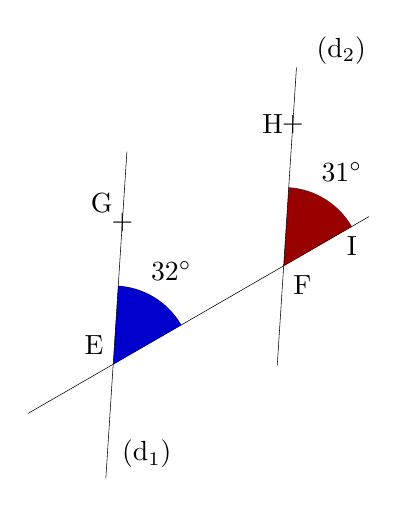
\begin{tikzpicture}[rotate=30,baseline=(C.base)]
        \coordinate[label=above left:E](A)at(0,0);
        \coordinate[label=below right:F](B)at(2.5,0);
        \coordinate[label=below:I](I)at(3.5,0);
        \coordinate[label=above left:G](C)at(1,1.5);
        \coordinate[label=left:H](D)at(3.5,1.5);
        \draw node at(C){+};
        \draw node at(D){+};
        \tkzFillAngle[fill=blue!80!black](B,A,C)
        \tkzLabelAngle[pos=1.4](B,A,C){$32^\circ$}
        \tkzFillAngle[fill=red!60!black](I,B,D)
        \tkzLabelAngle[pos=1.4](I,B,D){$31^\circ$}
        \tkzDrawLine[add=0.8 and 0.5](A,C)
        \tkzDrawLine[add=0.4 and 0.7](D,B)
        \tkzDrawLines[add=0.5 and 0.5](A,B)
        \draw node at(-0.2,-1.2){(d$_1$)};
        \draw node at(4.5,2){(d$_2$)};
    \end{tikzpicture}
    }}
\end{questions}

\end{document}